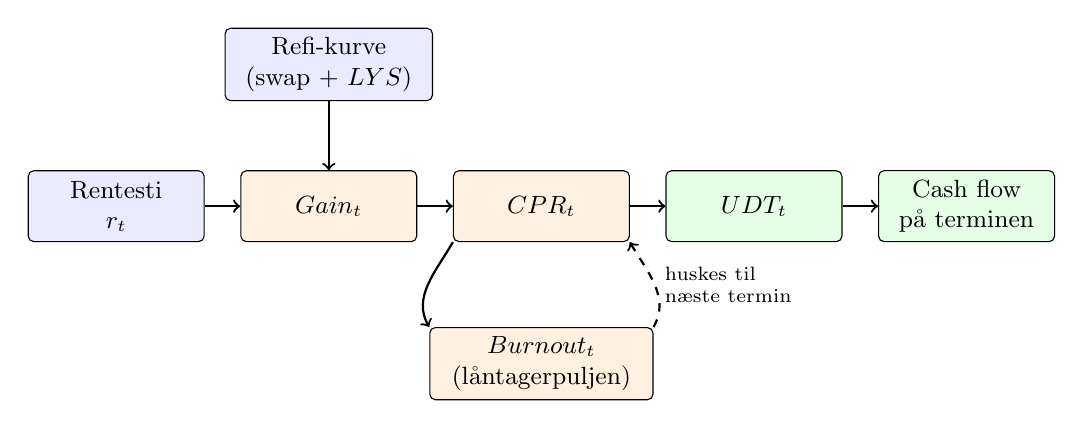
\begin{tikzpicture}[
    box/.style={draw, rounded corners=2pt, align=center, minimum height=9mm,
                text width=20mm, font=\small},
    rateb/.style={box, fill=blue!8},
    behav/.style={box, fill=orange!12},
    cfb/.style={box, fill=green!10},
    arr/.style={->, thick},
    darr/.style={->, thick, dashed}
]
\node[rateb] (r)   at (0,0)    {Rentesti\\\(r_t\)};
\node[behav] (g)   at (2.7,0)  {\(Gain_t\)};
\node[behav] (cpr) at (5.4,0)  {\(CPR_t\)};
\node[cfb]   (udt) at (8.1,0)  {\(UDT_t\)};
\node[cfb]   (cf)  at (10.8,0) {Cash flow\\på terminen};
\node[behav, text width=26mm] (b) at (5.4,-2.0) {\(Burnout_t\)\\(låntagerpuljen)};
\node[rateb, text width=24mm] (lys) at (2.7,1.8) {Refi-kurve\\(swap + \(LYS\))};

\draw[arr] (r) -- (g);
\draw[arr] (lys) -- (g);
\draw[arr] (g) -- (cpr);
\draw[arr] (cpr) -- (udt);
\draw[arr] (udt) -- (cf);
\draw[arr] (cpr.south west) to[out=-120,in=120] (b.north west);
\draw[darr] (b.north east) to[out=60,in=-60]
    node[right, font=\scriptsize, align=left] {huskes til\\næste termin}
    (cpr.south east);
\end{tikzpicture}
